\section{Результаты симуляций в модели канала IEEE 802.11ay <<Hotel Lobby>>}
\label{sec:simulations}
Эффективность разработанных алгоритмов была исследована с помощью численного
моделирования. Использовалась реалистичная модель канала на основе трассировки
лучей, описанная в стандарте IEEE 802.11ay  \cite{Maltsev2017}. Сценарий
<<Hotel Lobby>> рассматривался как базовый сценарий.
Параметры симуляции представлены в таб. \ref{tab:4.3}.
По умолчанию максимальное количество переотражений в процедуре
трассировки лучей установлено равным 2.

Обычный сценарий Hotel Lobby предоставляет канал с лучаом прямой видимости (LOS)
(см. рис. \ref{fig:4.30a}). Для того, чтобы убрать луч прямой видимости (NLOS),
посередине комнаты была установлена дополнительная стена
(см. рис. \ref{fig:4.30b}).

\begin{figure}[ht]
  \centering
  \begin{subfigure}{0.49\linewidth}
    \centering
    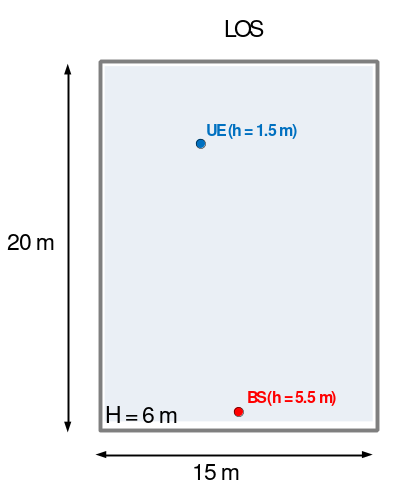
\includegraphics[width=\linewidth]{figs/fig4.30a}
    \caption{}
    \label{fig:4.30a}
  \end{subfigure}
  \begin{subfigure}{0.49\linewidth}
    \centering
    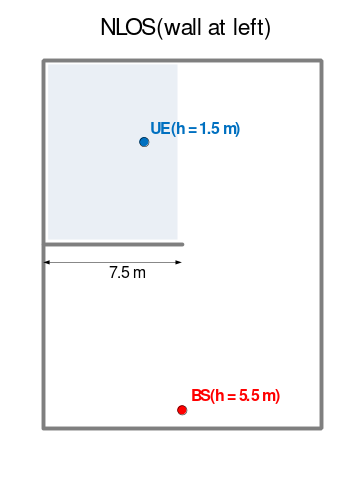
\includegraphics[width=0.88\linewidth]{figs/fig4.30b}
    \caption{}
    \label{fig:4.30b}
  \end{subfigure}
  \caption{Схема расположения БС и пользователя в сценариях (\subref{fig:4.30a}) LOS
    и (\subref{fig:4.30b}) NLOS}
  \label{fig:4.30}
\end{figure}
\begin{figure}[H]
  \centering
  \begin{subfigure}{0.49\linewidth}
    \centering
    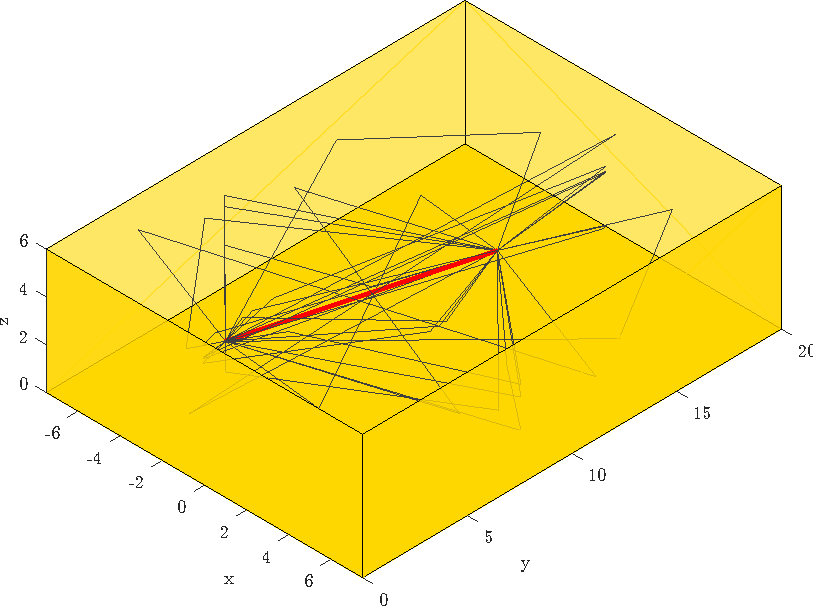
\includegraphics[width=\linewidth]{figs/4.30d.pdf}
    \caption{}
    \label{fig:4.30c}
  \end{subfigure}
  \begin{subfigure}{0.49\linewidth}
    \centering
    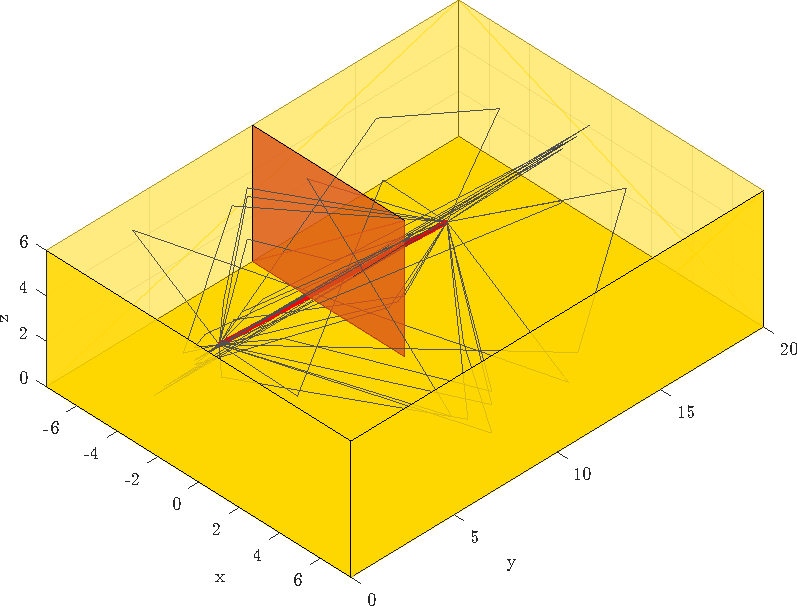
\includegraphics[width=\linewidth]{figs/4.30c.pdf}
    \caption{}
    \label{fig:4.30d}
  \end{subfigure}
  \caption{Геометрические лучи в сценариях (\subref{fig:4.30c}) LOS
    и (\subref{fig:4.30d}) NLOS. Красным цветом отмечен LOS-луч}
\end{figure}



В работе выполняется  Монте-Карло моделирование: пользователь вбрасывается
случайным образом в закрашенных синим областях на рис. \ref{fig:4.30}.
Обе антенные решетки пользователя лежат в горизонтальной плоскости.
Азимут всех вброшенных пользователей также определялся случайным образом.
Количество независимых экспериментов составило 10000.

Были рассмотрены 4 различных сценария:
\begin{enumerate}
  \item Статичный LOS канал
  \item Статичный NLOS канал
  \item Быстро изменяющийся NLOS канал
  \item Случай низкого ОСШ
\end{enumerate}

В случае быстро меняющегося канала пользователи вращались в горизонтальной
плоскости с угловой скоростью 100 град/с. Дополнительное описание
сценария c низким ОСШ приведено в разделе \ref{sec:singlepath:static:LOW-SNR}.
Другие параметры моделирования и системы приведены в таблице \ref{tab:4.10}.

\begin{table}
  \centering
  \caption{Параметры системы}
  \label{tab:4.10}
  \begin{tabular}{ll}
    \toprule
    \textbf{Параметр}                   & \textbf{Значение}              \\
    \midrule
    Окружение                           & IEEE 802.11ay Hotel Lobby      \\
    Несущая частота                     & 28 ГГц (FR2)                   \\
    Ширина полосы                       & 50 МГц                         \\
    Частота дискретизации               & 61.44 МГц                      \\
    Размер БПФ                          & 512                            \\
    Число используемых поднесущих       & 384                            \\
    Число поднесущих в пилотном сигнале & 127 (SS burst) или 32 (CSI-RS) \\
    Расстояние между поднесущими        & 120 кГц                        \\
    Температура шума                    & 300 K                          \\
    Мощность шума на поднесущую         & -114 дБм                       \\
    \bottomrule
  \end{tabular}
\end{table}

Для оценки точности оцененного AOA, производилось его сравнение  с эффективным азимутальным углом
\eqref{eq:4.2} некоторого геометрического луча из модели.
В случае однолучевых алгоритмов  это в качестве этого луча выбирался самый сильный
путь распространения. В представленных результатах разница между оцененным AOA и эффективным азимутом
геометрического луча отмечается как <<error>>.
Для оценки точности многолучевых алгоритмов  выполнялась более сложная процедура.
Во-первых, сортировался список геометрических лучей в порядке убывания коэффициента передачи.
Далее удалялись те лучи, которые находились в пределах ширины ДН вокруг самого сильного из них.
После этого следующий в списке лучей рассматривался как самый сильный и процедура повторялась до
конца всего списка.

Обозначим $\phi_1$ и $\phi_2$ как оценку AOA для основного и запасного лучей соответственно.
Пусть $\Psi$ -- список геометрических AOA, а $\psi_1$ —
АОА сильнейшего геометрического луча.
Ошибка определения основного луча $\psi_1$ определялась как наименьшая величина
между $\abs{\phi_1 - \psi_1}$ и  $\abs{\phi_2 - \psi_1}$.
Пусть наименьшая ошибка определилась на угле $\phi_1$ .
Ошибка определения запасного луча   $\min(\Psi - \phi_2)$,
т.е. ближайший геометрический луч будет считаться опорным для
резервного луча.

В качестве показателей эффективности рассматривались
следующие метрики:

\newcommand\CDF{\text{CDF}}
\begin{itemize}
  \item Функция распределения ошибки (\CDF) оценки AOA
  \item Среднеквадратичная ошибка (СКО)
  \item Среднее значение ошибки ($\CDF = 0.5$)
  \item Значение $\CDF$ по уровню 0.8 и 0.9
\end{itemize}

Предполагается, что алгоритмы работают, если ошибка меньше удвоенной ширины
ДН ($25,2^{\circ}$).  СКО учитывает только эксперименты, в которых
алгоритмы работают успешно.
Вероятность отказа работы алгоритма также измерялась.

Однолучевые  разработанные алгоритмы сравнивались с базовым алгоритмом
иерархического поиска (см.  раздел \ref{sec:hSearch}).  В случае многолучевости
базовая линия отсутствует.

Во всех случаях оценивалось типичное значение ОСШ, которое определялось
как отношение мощности сигнала и шума на одну поднесущую при идеальном
формировании луча.

\pgfplotstableset{
  col sep=semicolon, % the seperator in our .csv file
  every head row/.style={%
      output empty row,
      before row={\toprule%
          Алгоритм
          &\multicolumn{2}{c}{СКО, град}
          & $P_{fail}$
          &\multicolumn{2}{c}{CDF = 0.9, град}
          &\multicolumn{2}{c}{CDF = 0.8, град}
          &\multicolumn{2}{c}{CDF = 0.5, град}
          \\\midrule},
    },
  every last row/.style={after row=\bottomrule},
  string type,
}
\subsection{Однолучевые алгоритмы: стат. случай в LOS }


\begin{figure}[ht]
  \centering
  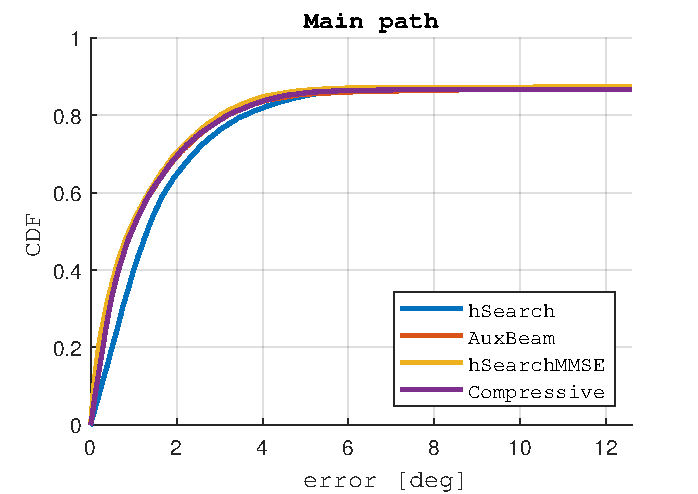
\includegraphics{results/rus/singlepath-static-LOS-1}
  \caption{Функция распределения (CDF) ошибки определения угла прихода. Стат. случай, LOS}
  \label{fig:singlepath:static:LOS}
\end{figure}

В первую очередь, однолучевые алгоритмы были протестированы в статическом LOS сценарии.
В качестве пилотного сигнала был выбран SS-burst, мощность передатчика $-15$ дБм.
ОСШ на одну поднесущую было от 10 до 40 дБ в большинстве случаев.
Приблизительно в 2\% случаев, ОСШ находилось в интервале от -10 дБ до 10 дБ.

Результаты моделирования представлены на рис. \ref{fig:singlepath:static:LOS} и
таб. \ref{tab:singlepath:static:LOS}. 
\begin{table}[h!]
  \begin{center}
    \caption{Стат. случай, LOS}
    \small
    \label{tab:singlepath:static:LOS}
    \pgfplotstabletypeset{results/rus/singlepath-static-LOS.csv} % filename/path to file
  \end{center}
\end{table}

По результатам моделирования видно, что все разработанные алгоритмы показывают 
схожие результаты и все они луче базовой линии (их кривые CDF находятся всегда
левее базовой кривой). Наличие ошибок в данном случае вызвано эффектом
замираний, приводящего к флуктуациям восстанавливаемого AOA относительно LOS
направления.  Замирания возникают из-за того, что помимо основного LOS луча,
рядом находятся также лучи, отраженные от потолка, пола, стены рядом с БС и
другие с первым порядком отражения, мощность не сильно меньше, чем у LOS луча.
Все эти лучи имеют разный эффективный азимут \eqref{eq:4.2}, поэтому в некоторых
измерениях восстанавливается не направление на главный луч, а направление на
один из лучей главного кластера. Это приводит к высокому значению <<ошибки>> 
для всех алгоритмов, превышающей теоретическую.

Также можно заметить, что в 13\% экспериментов ошибка оценки AOA составляет
более $25.2^\circ$ для всех алгоритмов. Это связано с <<краевым эффектом>>,
когда угол прихода близок к значению $\pm 90^\circ$ (см. рис. \ref{fig:4.5}).
Во-первых, эти направления равноправны с точки зрения волнового фронта и их
нельзя различить с помощью АР.  Это приводит к некоторым случайным скачкам около
$180^\circ$. Эта проблема может частично решаться с помощью кодовой книги, где
ни один луч не имеет направлений на $\pm 90^\circ$.  Во-вторых, при таких
значениях AOA появляется неоднозначность выбора между АР пользователя и поэтому
выбор АР становится случайным. В результате на функции распределения появляется 
некоторая <<полка>> (см. рис. \ref{fig:singlepath:static:LOSa}), вызванная этими
двумя эффектами.
\begin{figure}[ht]
  \centering
  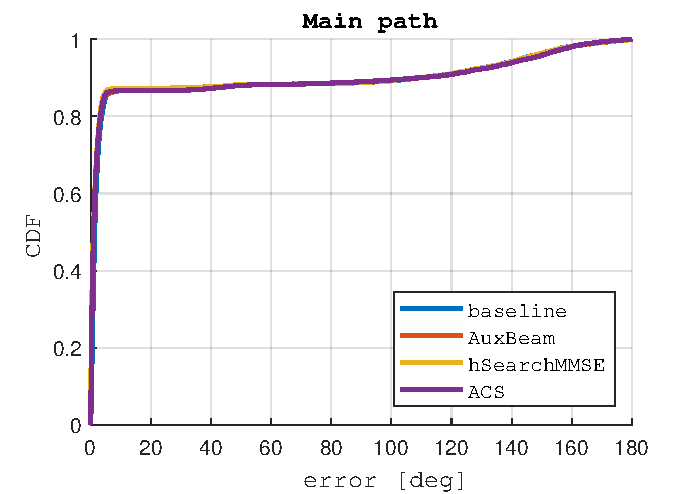
\includegraphics{results/rus/singlepath-static-LOS-full-1}
  \caption{Функция распределения (CDF) ошибки определения угла прихода. Стат. случай, LOS}
  \label{fig:singlepath:static:LOSa}
\end{figure}

\subsection{Однолучевые алгоритмы: стат. случай в NLOS }
\label{sec:singlepath:static:NLOS}

Также разработанные алгоритмы тестировались на статическом NLOS сценарии.
В качестве пилотного сигнала используется SS-burst, мощность передатчика равна -15 дБм.
ОСШ на поднесущую составляет от -5 до 20 дБ в большинстве случаев.
Приблизительно в 9\% случаев значение ОСШ находилось в диапазоне от -25 до -5 дБ.

Результаты моделирования представлены на рис. \ref{fig:singlepath:static:NLOS} и
таб. \ref{tab:singlepath:static:LOS}.  Иерархический поиск (\textit{baseline},
см. раздел \ref{sec:hSearch}) отмечен синим цветом, иерархический поиск с
минимизацией СКО (\textit{hSearchMMSE}, см. раздел
\ref{sec:hSearchMMSE:singlepath}) -- оранжевым, модифицированный алгоритм
моноимпульса (\textit{AuxBeam}, см. раздел \ref{sec:AuxBeam:singlepath}) --
красным цветом, адаптивный алгоритм бинарного поиска (\textit{ACS}, см. раздел
\ref{sec:ACS:singlepath}) -- фиолетовым.




\begin{figure}[ht]
  \centering
  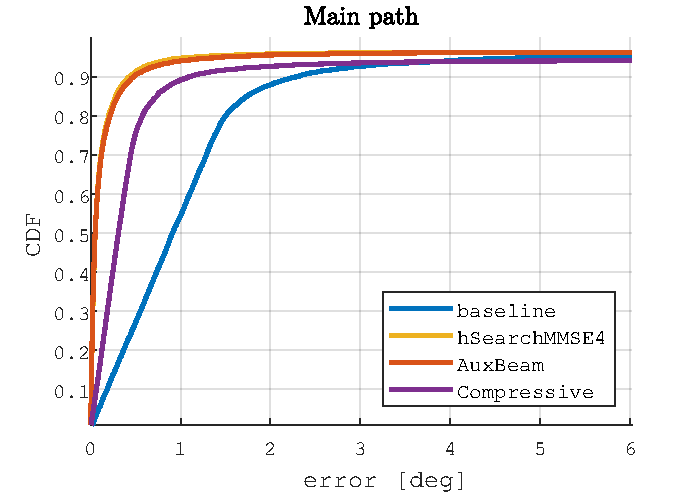
\includegraphics{results/rus/singlepath-static-NLOS-1}
  \caption{Функция распределения (CDF) ошибки определения угла прихода. Стат. случай, NLOS}
  \label{fig:singlepath:static:NLOS}
\end{figure}
\begin{table}[h!]
  \begin{center}
    \caption{Стат. случай, NLOS}
    \small
    \label{tab:singlepath:static:NLOS}
    \pgfplotstabletypeset{results/rus/singlepath-static-NLOS.csv} % filename/path to file
  \end{center}
\end{table}

В данном сценарии, разброс главного кластера геометрических лучей меньше, чем в
LOS, поэтому точность определения AOA выше. Лучшим решением в данном случае
являются \textit{AuxBeam} и \textit{hSearchMMSE}, поскольку они не имеют ошибки
квантования. Их функции распределения и другие метрики практически одинаковы.
\textit{ACS}-алгоритм имеет конечную ошибку квантования
$\Delta \psi = 0.0246 (\Delta \phi \approx 0.5^\circ)$, что и наблюдается в
результатах.  Также отметим, что несмотря на относительное низкое ОСШ на одну
поднесущую, точность представленных алгоритмов достаточно высоки. Это происходит
из-за усреденения по 127 пилотным поднесущим в SS-burst.

\subsection{Однолучевые алгоритмы: быстро меняющийся канал }
\label{sec:singlepath:rotation:NLOS}
Интересным случаем является быстро меняющийся NLOS канал. Мощность перелатчика
равна 23 дБм.  ОСШ на поднесущую в большинстве случаев составляет от 30 до 60
дБ. Примерно в 3\% случаев ОСШ находится в диапазоне от 10 до 30 дБ.

\begin{figure}[ht]
  \centering
  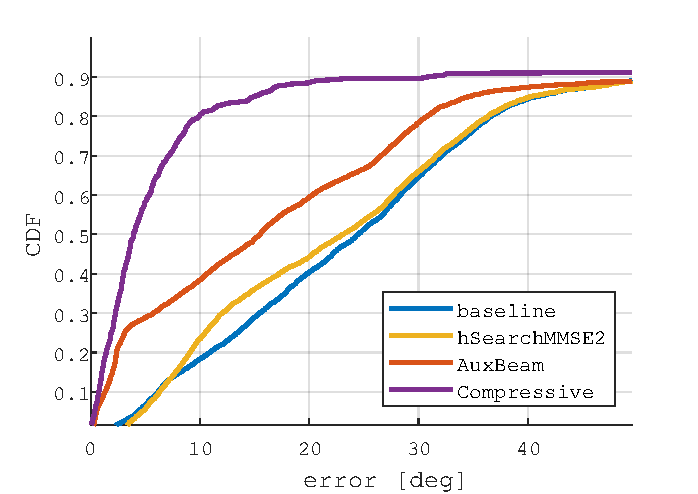
\includegraphics{results/rus/singlepath-rotation-NLOS-1}
  \caption{Функция распределения (CDF) ошибки определения угла прихода. Динам. случай, NLOS, SS-burst}
  \label{fig:singlepath:rotation:NLOS-1}
\end{figure}
Результаты симуляции представлены на рис.\ref{fig:singlepath:static:NLOS} и
таб.  \ref{tab:singlepath:static:NLOS}.
Для SS-burst с периодом 20 мс процедура сканирования для этого сценария слишком долгая --
от 300 до 380 мс, что соответствует углу поворота от 30 до 38 градусов (ширина ДН $12.6^\circ$).
Лучше всего работает \textit{ACS}-алгоритм, поскольку на начальных этапах
он использует широкую ДН, устойчивую к вращению пользователя. 

Остальные алгоритмы работают плохо и ошибка оказывается равномерно
распределенной в пределах поворота пользователя за время измерения.  В среднем,
продолжительность \textit{AuxBeam} меньше, чем \textit{hSearchMMSE}, что дает
ему преимущество. Стоит отметить, что в 25 \% случаев ошибка \textit{AuxBeam}
менее 3 град. Это соответствует начальным условиям, когда фактический AOA
находится между двумя последними прозвоненными лучами и полученные измерения не успевают
устареть.

Эффективность \textit{hSearchMMSE} немного выше базового алгоритма, в силу 
его меньшей длительности: на этапе дополнительный измерений измерялись только 2 луча,
т.е. общее количество измеренных лучей равно 18, в то время как у \textit{baseline} --
20. Стоит отметить, что этап дополнительных измерений после процедуры SLS, работает по сильно 
устаревшим данным, что делает саму процедуру почти бесполезной. 

Гораздо лучшее решение предоставляется с помощью CSI-RS (см. рис.
\ref{fig:singlepath:rotation:NLOS-1} и таб. \ref{tab:singlepath:static:NLOS})в
качестве пилотных сигналов. Продолжительность прозвонки в этом случае составляет
от 32 до 40 мс, что соответствует повороту пользователя на 3.2 - 4.0 град.

В этом случае наилучшее решение дает алгоритм \AuxBeam. Это происходит поскольку
его длительность одна из самых низких. 
\ACS алгоритм несмотря на такую же длительность работает значительно хуже, 
поскольку у него есть ошибка квантования.
\hSearchMMSE, несмотря на свою длительность, не имеют ошибки квантования и его 
эффективность во многих случаях совпадает с \AuxBeam.
\begin{table}[h!]
  \begin{center}
    \caption{Динам. случай, NLOS, SS-burst}
    \small
    \label{tab:singlepath:rotation:NLOS}
    \pgfplotstabletypeset{results/rus/singlepath-rotation-NLOS.csv} % filename/path to file
  \end{center}
\end{table}

\begin{figure}[ht]
  \centering
  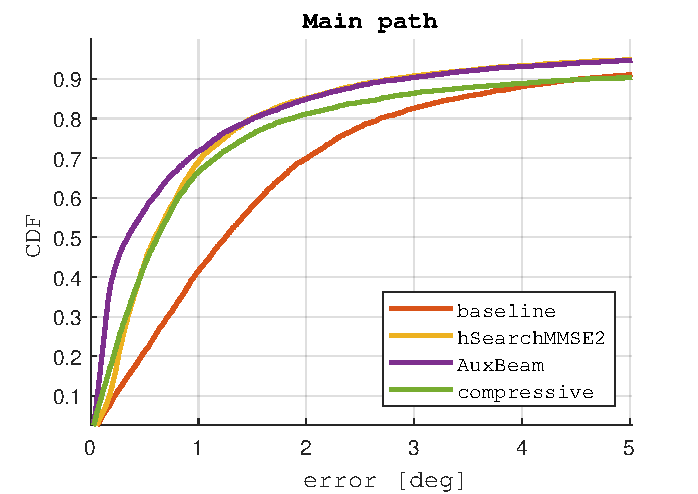
\includegraphics{results/rus/singlepath-rotation-NLOS-CSI-RS-1}
  \caption{Функция распределения (CDF) ошибки определения угла прихода. Динам. случай, NLOS, CSI-RS}
  \label{fig:singlepath:rotation:NLOS-2}
\end{figure}

\begin{table}[h!]
  \begin{center}
    \caption{Динам. случай, NLOS, CSI-RS}
    \small
    \label{tab:singlepath:rotation:NLOS-2}
    \pgfplotstabletypeset{results/rus/singlepath-rotation-NLOS-2.csv} % filename/path to file
  \end{center}
\end{table}

\subsection{Однолучевые алгоритмы: низкое ОСШ}
\label{sec:singlepath:static:LOW-SNR}
Чтобы протестировать алгоритмы в сценарии с низким ОСШ, 
большинство лучей были заблокированны с помощью дополнительной стены так, чтобы
пользователь находился в отдельном помещении. 

В симуляции моделировались отражения до 4-го порядка.
В этом случае <<самый сильный>> луч входит в комнату
через <<дверь>> и достигает пользователя после четырехкратного отражения. Геометрия
представлена на рис. \ref{fig:4.36} (более слабые лучи тоже присутствуют в
симуляции, но они не изображены на рисунке).
Положение пользователя было зафиксировано. Ориентация пользователя в горизонтальной плоскости была
случайной.

\begin{figure}[ht]
  \centering
  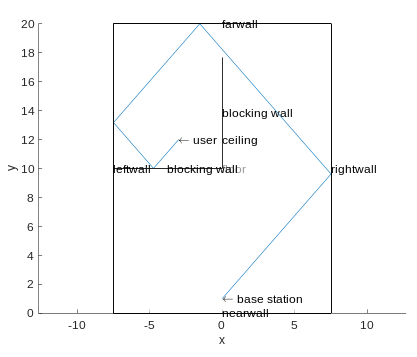
\includegraphics[width=.5\linewidth]{figs/fig4.36}
  \caption{Геометрия симуляций для случая низкого ОСШ}
  \label{fig:4.36}
\end{figure}

Мощность передатчика равна -10 дБм. ОСШ на одну поднесущую находится в диапазоне
от -47 до -25 дБ. В качестве опорного сигнала выбран SS-burst. 

Результаты симуляции представлены на рис.\ref{fig:singlepath:static:LOW-SNR} и
таб.  \ref{tab:singlepath:static:LOW-SNR}.  Иерархический поиск (\baseline, см.
раздел \ref{sec:hSearch}) отмечен синим цветом, разработанный иерархический
поиск с минимизацией СКО (\hSearchMMSE, см. раздел
\ref{sec:hSearchMMSE:singlepath}) -- оранжевым $(M=2)$ и зеленым $(M=4)$,
модифицированный алгоритм моноимпульса (\AuxBeam, см. раздел
\ref{sec:AuxBeam:singlepath}) -- красным цветом, адаптивный алгоритм бинарного
поиска (\ACS, см. раздел \ref{sec:ACS:singlepath}) -- фиолетовым.
\begin{figure}[ht]
  \centering
  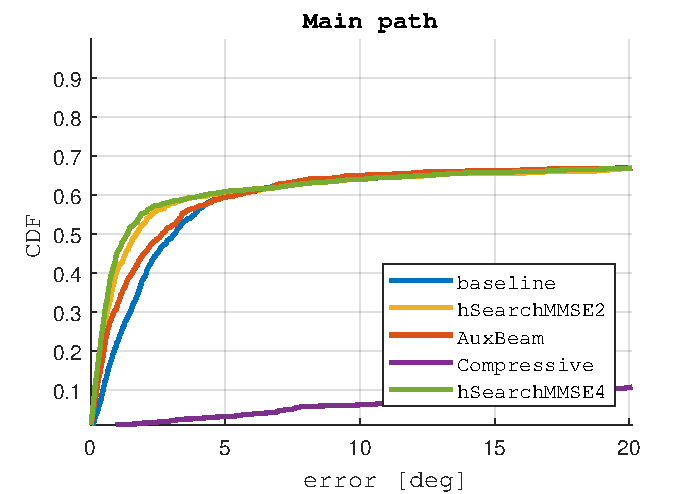
\includegraphics{results/rus/singlepath-static-LOW-SNR-1}
  \caption{Функция распределения (CDF) ошибки определения угла прихода. Стат. случай, LOS, основной луч}
  \label{fig:singlepath:static:LOW-SNR}
\end{figure}

\begin{table}[h!]
  \begin{center}
    \caption{Низкое ОСШ}
    \small
    \label{tab:singlepath:static:LOW-SNR}
    \pgfplotstabletypeset{results/rus/singlepath-static-LOW-SNR.csv} % filename/path to file
  \end{center}
\end{table}


Из результатов моделирования видно, все алгоритмы, кроме \ACS работают хорошо в
68\% случаев. При этом практически все алгоритмы проигрывают \baseline в
значении СКО (кроме \AuxBeam). Наличие высоких ошибок оценки
АОА не позволяют дать точную оценку СКО для приемлемого количества
экспериментов. С точки зрения медианного значения ошибки $(CDF = 0,5)$
кажется более подходящей метрикой. Оба варианта \hSearchMMSE и \AuxBeam
превосходят базовый уровень по этому показателю.  Мы видим, что наилучшее
решение дает алгоритм \hSearchMMSE $(M = 4)$.  

Наихудшим решением в случае низкого ОСШ является \ACS. На самом деле, этот
алгоритм в данном случае не оценивает AOA, а лишь возвращает равномерно
распределенное сдучайное значение. Это вызвано тем, что \ACS на первых двух
итерациях использует широкие ДН, что приводит низкому усилению АР и высокой
вероятности ошибки в выборе начального сектора. 


\pgfplotstableset{
  fixed zerofill,
  col sep=semicolon, % the seperator in our .csv file
  string type,
  precision=2,
  every last row/.style={after row=\bottomrule},
  every head row/.style={
      before row={\toprule},
      after row={
          \midrule},
    }
}
\subsection{Многолучевые алгоритмы: стат. случай в LOS}

Многолучевые алгоритмы были протестированы в статическом LOS сценарии. В
качестве опорного сигнала использовался SS-burst.  Мощность передатчика была
установлена равной 10 дБм. ОСШ на поднесущую
составляло от 35 до 65 дБ в подавляющем большинстве случаев. Примерно в 3\%
случаев значение ОСШ находилось в диапазоне от 19 до 35 дБ.  

Полученные результаты моделирования и показатели эффективности для основного
луча представлены на рис. \ref{fig:multipath:static:LOS:1}  и таб.
\ref{fig:multipath:static:LOS:1}. Полученные результаты моделирования и
показатели эффективности запасного луча представлены на рис.
\ref{fig:multipath:static:LOS:2} и в таб. \ref{tab:multipath:static:LOS:2}.
\begin{figure}[H]
  \centering
  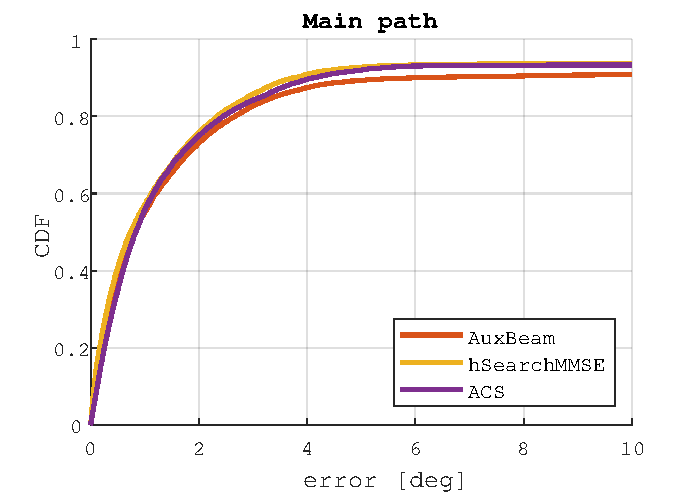
\includegraphics{results/rus/multipath-static-LOS-1}
  \caption{Функция распределения (CDF) ошибки определения угла прихода. Стат. случай, LOS, основной луч}
  \label{fig:multipath:static:LOS:1}
\end{figure}
\begin{table}[H]
  \begin{center}
    \caption{Стат. случай, LOS, основной луч}
    \label{tab:multipath:static:LOS:1}
    \pgfplotstabletypeset{results/rus/multipath-static-LOS-1.csv}
  \end{center}
\end{table}
Для оценки угла прихода основного луча \AuxBeam, \hSearchMMSE и \ACS показывают
почти одинаковую эффективность. Тот же результат
наблюдался и в случае однолучевых версий алгоритмов. 

Для резервного луча \hSearchMMSE в 10\% случаев не нашел луча или он был ассоциирован 
с основным лучом. Подобные случаи исключались из набора данных в CDF и таблицах.
Для \AuxBeam это значение составило 5\%, для \ACS -- 47\%. Такой плохой результат 
\ACS связан прежде всего с эффектом утечки мощности главного луча через 
боковые лепестки ДН. 

По результатам моделирования можно сделать вывод, что 
\AuxBeam и \hSearchMMSE позволяют достаточно хорошо оценить направление на 
запасной луч.  

\begin{figure}[H]
  \centering
  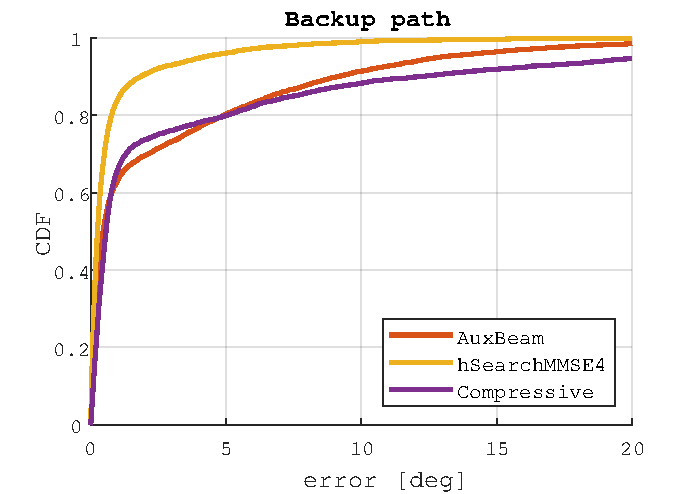
\includegraphics{results/rus/multipath-static-LOS-2}
  \caption{Функция распределения (CDF) ошибки определения угла прихода. Стат. случай, LOS, запасной луч}
  \label{fig:multipath:static:LOS:2}
\end{figure}
\begin{table}[H]
  \begin{center}
    \caption{Стат. случай, LOS, запасной луч}
    \label{tab:multipath:static:LOS:2}
    \pgfplotstabletypeset{results/rus/multipath-static-LOS-2.csv}
  \end{center}
\end{table}

\subsection{Многолучевые алгоритмы: стат. случай в NLOS }
\begin{figure}[H]
  \centering
  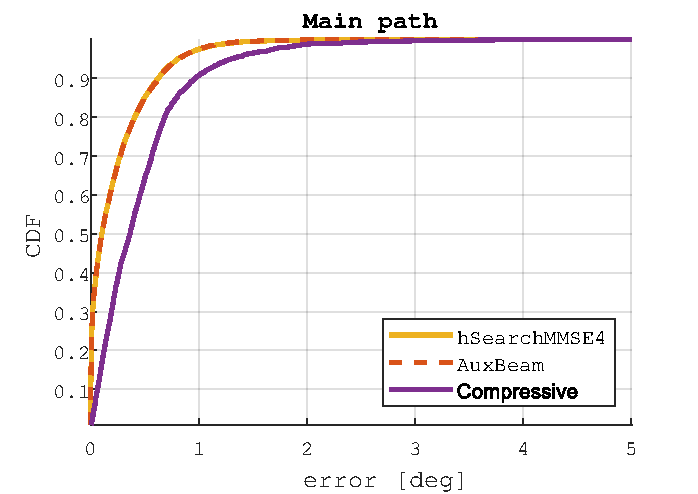
\includegraphics{results/rus/multipath-static-NLOS-1}
  \caption{Функция распределения (CDF) ошибки определения угла прихода. Стат. случай, NLOS, основной луч}
  \label{fig:multipath:static:NLOS:1}
\end{figure}

\begin{table}[H]
  \begin{center}
    \caption{Стат. случай, NLOS, основной луч}
    \label{tab:multipath:static:NLOS:1}
    \pgfplotstabletypeset{results/rus/multipath-static-NLOS-1.csv}
  \end{center}
\end{table}

\begin{table}[H]
  \begin{center}
    \caption{Стат. случай, NLOS, запасной луч}
    \label{tab:multipath:static:NLOS:2}
    \pgfplotstabletypeset{results/rus/multipath-static-NLOS-2.csv}
  \end{center}
\end{table}
\begin{figure}[H]
  \centering
  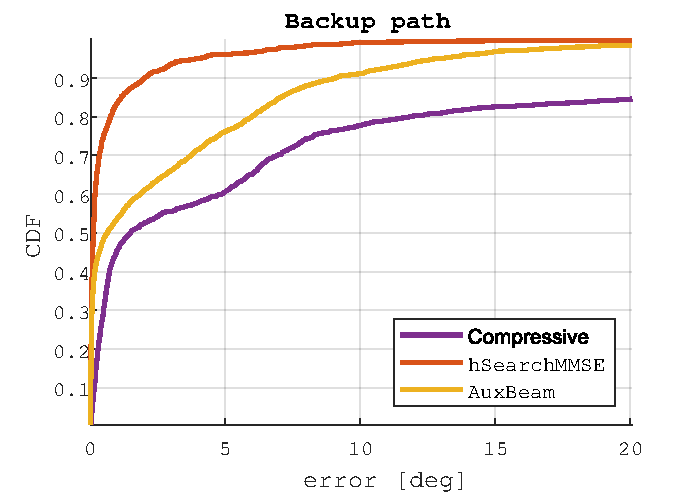
\includegraphics{results/rus/multipath-static-NLOS-2}
  \caption{Функция распределения (CDF) ошибки определения угла прихода. Стат. случай, NLOS, запасной луч}
  \label{fig:multipath:static:NLOS:2}
\end{figure}

\subsection{Многолучевые алгоритмы: быстро меняющийся канал}
Другим интересным сценарием является быстро меняющийся канал NLOS. Здесь были
приняты во внимание аналогичные результаты однолучевых алгоритмов (см. раздел
\ref{sec:singlepath:rotation:NLOS}) и использовался только CSI-RS.  Мощность
передатчика устанавливалась равным 23 дБм.  Отношение сигнал-шум на поднесущую в
подавляющем большинстве случаев составляло от 25 до 55 дБ.  Примерно в 3\%
случаев значение SNR находилось в диапазоне от 10 до 25 дБ.

Полученные результаты моделирования и показатели эффективности для основного луча представлены на
рис. \ref{fig:multipath:rotation:NLOS:1} и в таб. \ref{tab:multipath:rotation:NLOS:1}. 
Полученные результаты моделирования и показатели эффективности для резервного
луча представлены на рис. \ref{fig:multipath:rotation:NLOS:2} и в таб. \ref{tab:multipath:rotation:NLOS:2}.
\begin{figure}[H]
  \centering
  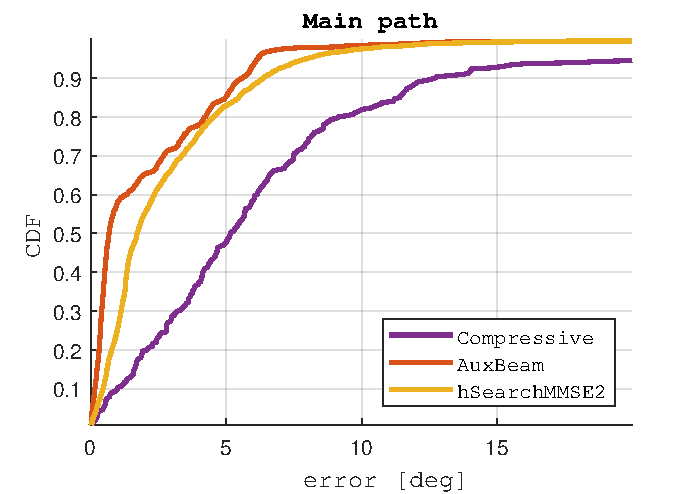
\includegraphics{results/rus/multipath-rotation-NLOS-1}
  \caption{Функция распределения (CDF) ошибки определения угла прихода. Динам. случай, NLOS, основной луч}
  \label{fig:multipath:rotation:NLOS:1}
\end{figure}

\begin{table}[H]
  \begin{center}
    \caption{Динам. случай, NLOS, основной луч}
    \label{tab:multipath:rotation:NLOS:1}
    \pgfplotstabletypeset{results/rus/multipath-rotation-NLOS-1.csv}
  \end{center}
\end{table}

\begin{figure}[H]
  \centering
  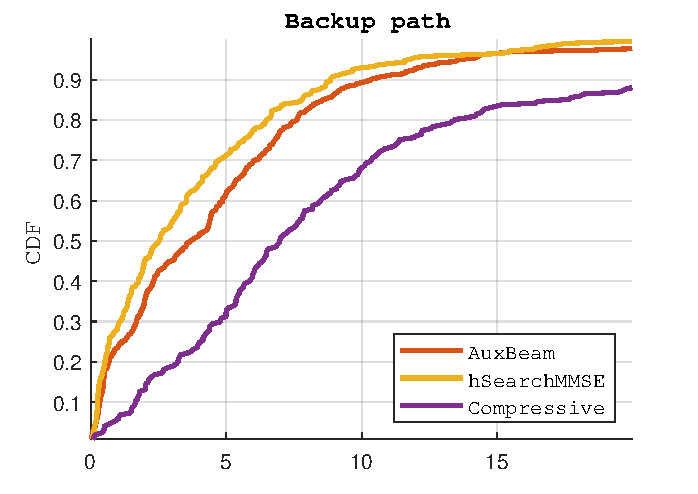
\includegraphics{results/rus/multipath-rotation-NLOS-2}
  \caption{Функция распределения (CDF) ошибки определения угла прихода. Динам. случай, NLOS, запасной луч}
  \label{fig:multipath:rotation:NLOS:2}
\end{figure}

\begin{table}[H]
  \begin{center}
    \caption{Динам. случай, NLOS, запасной луч}
    \label{tab:multipath:rotation:NLOS:2}
    \pgfplotstabletypeset{results/rus/multipath-rotation-NLOS-2.csv} % filename/path to file
  \end{center}
\end{table}


Длительность алгоритмов находится в диапазоне от 32 до 64 мс, что соответствует повороту на 3.2 - 6.4 град.
Мы снова видим, что наилучшее решение для основного луча дает кратчайший алгоритм, т.е.
\AuxBeam (требуется 32-40 мс). Второй результат показывает \hSearchMMSE, продолжительность которого составляет
40 мс (всегда прозванивается два дополнительных луча на этапе уточнения). 

Что касается резервного луча, то наибольшую эффективность обеспечивает \hSearchMMSE в силу своей короткой длительности 
и большей гибкости по сравнению с \AuxBeam.
\ACS не нашел резервный путь в 26\% всех случаев. Эти случаи
были исключены из набора данных для получения CDF и метрик. Для других алгоритмов эти значения были
менее 0.5\%.

\subsection{Многолучевые алгоритмы: низкое ОСШ}
Многолучевые алгоритмы были протестированы в статическом сценарии NLOS с низким
ОСШ. В качестве опорный сигнала был выбран SS-burst. 
Мощность передатчика была установлена равной -25
дБм. Отношение сигнал-шум на поднесущую составило от -30 до 5 дБ в
большинстве случаев. Примерно в 3\% случаев значение ОСШ находилось в
диапазоне от -80 до -30 дБ.

Полученные результаты моделирования для основного луча представлены на
рис.\ref{fig:multipath:static:LOW-SNR:1} и 
таб.\ref{tab:multipath:static:LOW-SNR:1}. Результаты моделирования для
резервного пути представлены на рис. \ref{fig:multipath:static:LOW-SNR:2} и таб.
\ref{tab:multipath:static:LOW-SNR:2}.

\begin{figure}[H]
  \centering
  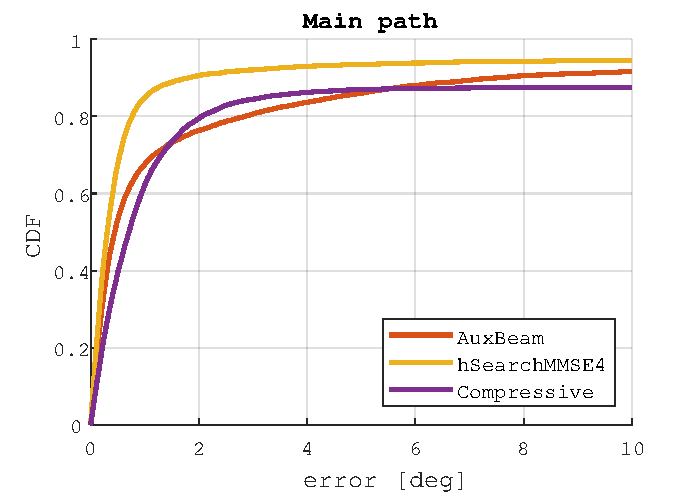
\includegraphics{results/rus/multipath-static-LOW-SNR-1}
  \caption{Функция распределения (CDF) ошибки определения угла прихода. Низкое ОСШ, основной луч}
  \label{fig:multipath:static:LOW-SNR:1}
\end{figure}

\begin{table}[H]
  \begin{center}
    \caption{Низкое ОСШ, основной луч}
    \label{tab:multipath:static:LOW-SNR:1}
    \pgfplotstabletypeset{results/rus/multipath-static-NLOS-1.csv}
  \end{center}
\end{table}

\begin{figure}[H]
  \centering
  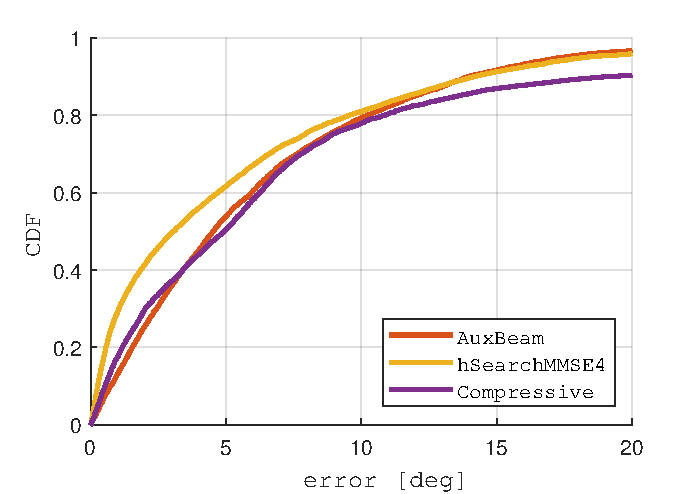
\includegraphics{results/rus/multipath-static-LOW-SNR-2}
  \caption{Функция распределения (CDF) ошибки определения угла прихода. Низкое ОСШ, запасной луч}
  \label{fig:multipath:static:LOW-SNR:2}
\end{figure}

\begin{table}[H]
  \begin{center}
    \caption{Низкое ОСШ, запасной луч}
    \label{tab:multipath:static:LOW-SNR:2}
    \pgfplotstabletypeset{results/rus/multipath-static-NLOS-2.csv} % filename/path to file
  \end{center}
\end{table}

Как и ожидалось, наилучшее решение дает алгоритм \hSearchMMSE, который
является аппроксимацией алгоритма Фурье и не имеет ошибки квантования. Что
касается других алгоритмов, \ACS не
нашел резервный путь в 53\% случаев, в то время как  для \AuxBeam и \hSearchMMSE 
это значение составило 1-3\%.  Эти случаи были исключены из набора
данных для получения CDF и таблиц. Также следует отметить, что \AuxBeam
более подвержен влиянию низкого ОСШ по сравнению с \hSearchMMSE. 
Это связано с нестабильностью метрики \eqref{eq:4.39}, особенно в случаях, когда 
сигнал подавляется ДН элементов АР, что ведет к чрезвычайно низкому ОСШ.